\documentclass[11pt]{article}

\usepackage[margin=1in]{geometry}
\usepackage[T1]{fontenc}
\usepackage{lmodern}
\usepackage{amsmath,amssymb,amsthm}
\usepackage{graphicx}
\usepackage{booktabs}
\usepackage{multirow}
\usepackage{array}
\usepackage{xcolor}
\usepackage{hyperref}
\usepackage{caption}
\usepackage{subcaption}
\usepackage{enumitem}
\usepackage{listings}
\usepackage{microtype}
\usepackage{float}
\usepackage{tikz}
\usetikzlibrary{arrows.meta,positioning,calc,decorations.pathreplacing,decorations.pathmorphing,angles,quotes}
\usepackage{tcolorbox}
\tcbuselibrary{breakable,skins}

\newtcolorbox{intuition}[1][]{
  enhanced,breakable,colback=blue!4,colframe=blue!45!black,
  title=Intuition,fonttitle=\bfseries,left=4pt,right=4pt,top=4pt,bottom=4pt,#1}
\newtcolorbox{pitfall}[1][]{
  enhanced,breakable,colback=red!3,colframe=red!55!black,
  title=Common pitfall,fonttitle=\bfseries,left=4pt,right=4pt,top=4pt,bottom=4pt,#1}
\newtcolorbox{recipe}[1][]{
  enhanced,breakable,colback=green!3,colframe=green!45!black,
  title=Recipe,fonttitle=\bfseries,left=4pt,right=4pt,top=4pt,bottom=4pt,#1}

\hypersetup{
  colorlinks=true,
  linkcolor=blue!50!black,
  citecolor=blue!50!black,
  urlcolor=blue!50!black
}

\graphicspath{{figures/}}

\lstset{
  basicstyle=\ttfamily\small,
  breaklines=true,
  frame=single,
  backgroundcolor=\color{gray!6},
  keywordstyle=\color{blue!60!black},
  commentstyle=\color{green!40!black},
  stringstyle=\color{red!50!black},
  showstringspaces=false,
  columns=fullflexible,
  keepspaces=true
}

\newcommand{\bx}{\mathbf{x}}
\newcommand{\bq}{\mathbf{q}}
\newcommand{\bu}{\mathbf{u}}
\newcommand{\bA}{\mathbf{A}}
\newcommand{\bB}{\mathbf{B}}
\newcommand{\bQ}{\mathbf{Q}}
\newcommand{\bR}{\mathbf{R}}

\title{\textbf{Chapter 4 Assignment}\\[4pt]
Simple Models of Walking and Running}
\author{Zihao Liu\\[2pt]
Student ID: 220261979\\[2pt]
\texttt{213222647@seu.edu.cn}}
\date{October 2026}

\begin{document}
\maketitle

\begin{abstract}
This report covers Chapter 4 of the course.  Part~I comments on the four
textbook examples: the rimless wheel (Example~4.3), the compass gait
(Example~4.4), the SLIP simulation (Example~4.5) and the SLIP apex-to-apex map
(Example~4.6).  The supplied notebooks were run, the results are interpreted
with the theory of hybrid and passive-dynamic locomotion, and sensitivity
studies on slope, initial conditions, energy and touchdown angle are reported.
Part~II solves the Section~4.6 exercise: the one-dimensional hopper.  The
energy analysis is carried out, the hopping controller is implemented, and the
autograder gives $13/13$.  The complete Python code and notebooks accompany the
submission; the most important code is reproduced here.
\end{abstract}

\tableofcontents
\newpage

%=====================================================================
\section{Overview and Reproducibility}
%=====================================================================

The assignment consists of:
\begin{itemize}[leftmargin=1.5em]
  \item \textbf{Examples} (code supplied; run and comment): Examples~4.3,
        4.4, 4.5 and 4.6.
  \item \textbf{Section 4.6} (all exercises): the one-dimensional hopper.
\end{itemize}

\begin{sloppypar}
All simulations use Drake 1.58.0 and the \texttt{underactuated} package
2026.9.8 in \texttt{/Users/leo/venvs/drake/bin/python} (NumPy 2.5.4,
SciPy 1.18.1, Matplotlib 3.11.2).  The notebooks were executed headlessly with
\texttt{COLAB\_TESTING=1}, which prevents the MeshCat visualizer from blocking.
\end{sloppypar}

\begin{center}
\begin{tabular}{ll}
\toprule
Contents & Location \\
\midrule
Example notebooks & \texttt{Ch-4/Exp4'3-*.ipynb}, \texttt{Exp4'4-*.ipynb}, \\
 & \texttt{Exp4'5-6-slip.ipynb} \\
Section 4.6 notebook & \texttt{Ch-4/Exp4'6-one\_d\_hopper.ipynb} \\
Analysis scripts and figures & \texttt{Ch-4/exp4\_analysis/} \\
This report & \texttt{Ch-4/Ch4\_Assignment\_Report/} \\
\bottomrule
\end{tabular}
\end{center}

The Section~4.6 autograder result is
\begin{center}
\texttt{Total score is 13/13.}
\end{center}

\subsection*{How to read this report}

The report has three layers: \emph{models}, \emph{simulations} and
\emph{interpretation}.  If an equation looks dense, read the
\textbf{Intuition} boxes first: they give the physical picture without
algebra.  The \textbf{Recipe} boxes summarise a reusable procedure, and the
\textbf{Common pitfall} boxes point out the mistakes that are easy to make in
hybrid locomotion.

\begin{center}
\small
\begin{tabular}{p{0.16\textwidth}p{0.39\textwidth}p{0.37\textwidth}}
\toprule
Part & What is done & What to look for \\
\midrule
Example 4.3 & Rimless wheel simulation, return map & collision loss vs.\
gravity input; stable fixed point; critical slope \\
Example 4.4 & Compass gait simulation & passive limit cycle; step-to-step
map; narrow basin of attraction \\
Example 4.5 & SLIP simulation & flight/stance phases; no collision loss;
energy conservation \\
Example 4.6 & SLIP apex-to-apex map & 1D map on an energy slice; stable and
unstable fixed points; partial stability \\
Section 4.6 & One-dimensional hopper & energy balance; preload at the bottom;
reset at the apex; hopping-height tracking \\
\bottomrule
\end{tabular}
\end{center}

\begin{intuition}[breakable=false,title={The big picture in five sentences}]
Walking and running are \emph{periodic} motions, not motions to a fixed
point.  The right object is therefore a \emph{limit cycle} and its
\emph{step-to-step} (Poincar\'e) map.  A fixed point of that map is a periodic
gait; the slope of the map at the fixed point decides whether the gait is
stable.  Passive walkers get their energy from gravity on a slope and lose it
at foot strike; running models such as SLIP have no impact loss but store
energy in a spring.  In all cases, the low-dimensional map is the key to both
understanding and control.
\end{intuition}

\begin{center}
\small
\begin{tabular}{ll}
\toprule
Symbol & Meaning \\
\midrule
$\alpha$ & half-angle between adjacent spokes (rimless wheel) \\
$\gamma$ & slope of the ramp \\
$\omega=\dot\theta$ & angular velocity in the support phase \\
$\omega^*$ & fixed point of the return map (periodic gait) \\
$\theta_{st},\theta_{sw}$ & stance and swing leg angles (compass gait) \\
$\theta_{td}$ & touchdown angle of the SLIP leg \\
$z$ & apex height (SLIP) \\
$P(z)$ & apex-to-apex return map \\
$\bar\delta$ & hopping preload (Section 4.6) \\
\bottomrule
\end{tabular}
\end{center}

%=====================================================================
\section{Example 4.3: The Rimless Wheel}
%=====================================================================

\subsection{Model and hybrid dynamics}

The rimless wheel is a rigid wheel with $n=8$ spokes, no rim, and a point mass
$m$ at the hip.  The half-angle between adjacent spokes is
$\alpha=\pi/8$, the radius is $l=1$ m, and the wheel rolls down a ramp of slope
$\gamma$.  The stance phase is a simple pendulum:
\begin{equation}
\ddot\theta=\frac{g}{l}\sin\theta,
\end{equation}
where $\theta$ is measured from the vertical and $\theta=0$ is the unstable
upright position.  Between impacts the mechanical energy
\begin{equation}
E=\frac12ml^2\dot\theta^2+mgl\cos\theta
\end{equation}
is conserved.

At each foot strike the new spoke becomes the stance leg.  Angular momentum
about the new contact point is conserved, while the collision is inelastic:
\begin{equation}
\dot\theta^+=\dot\theta^-\cos(2\alpha).
\end{equation}
The kinetic energy is multiplied by $\cos^2(2\alpha)$; for $\alpha=\pi/8$
this is $1/2$, i.e.\ half of the kinetic energy is lost at every step.

\begin{figure}[htbp]
\centering
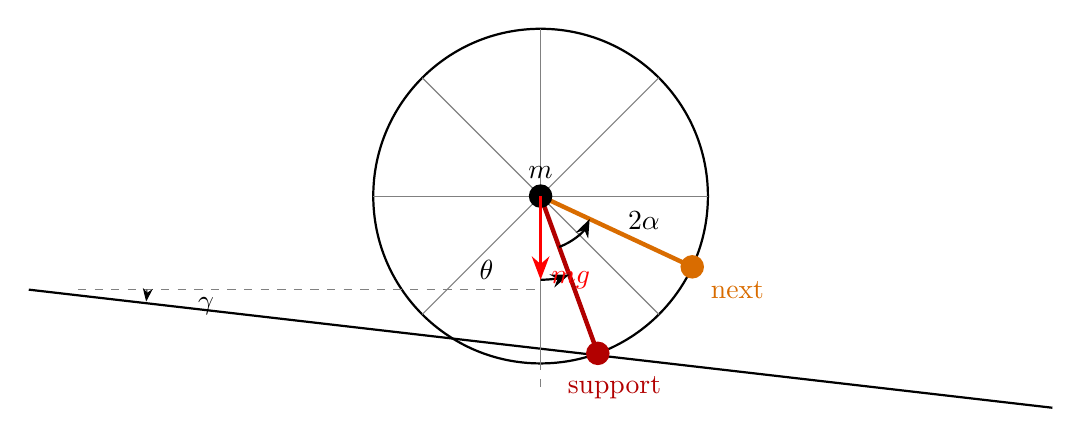
\begin{tikzpicture}[>=Stealth,scale=1.25]
  \draw[thick] (-5.2,0.75)--(5.2,-0.45);
  \coordinate (C) at (0,1.7);
  \draw[thick] (C) circle (1.7);
  \foreach \a in {-90,-45,0,45,90,135,180,225}
    \draw[gray] (C)--++(\a:1.7);
  \draw[ultra thick,red!70!black] (C)--++(-70:1.7);
  \draw[ultra thick,orange!85!black] (C)--++(-25:1.7);
  \fill (C) circle (3.4pt) node[above=3pt] {$m$};
  \fill[red!70!black] (C)++(-70:1.7) circle (3.4pt);
  \fill[orange!85!black] (C)++(-25:1.7) circle (3.4pt);
  \draw[dashed,gray] (C)--++(0,-2.0);
  \draw[->,thick] (C)++(-90:0.85) arc[start angle=-90,end angle=-70,radius=0.85];
  \node at (-0.55,0.95) {$\theta$};
  \draw[->,thick] (C)++(-70:0.55) arc[start angle=-70,end angle=-25,radius=0.55];
  \node at (1.05,1.45) {$2\alpha$};
  \draw[->,very thick,red] (C)--++(0,-0.85) node[right] {$mg$};
  \node[red!70!black] at (0.75,-0.25) {support};
  \node[orange!85!black] at (2.0,0.75) {next};
  \draw[dashed,gray] (-4.7,0.75)--(0,0.75);
  \draw[->] (-4.0,0.75) arc[start angle=0,end angle=-7,radius=1.0];
  \node at (-3.4,0.58) {$\gamma$};
\end{tikzpicture}
\caption{Rimless-wheel schematic.  The wheel has $n=8$ spokes, so the angle
between adjacent spokes is $2\alpha=\pi/4$.  The support spoke is the one
currently on the ground; the next spoke is the one that will strike next.
Gravity acts at the hub mass $m$.}
\label{fig:rimless_wheel}
\end{figure}

\begin{intuition}[breakable=false,title={Why a wheel without a rim can keep walking}]
At every step the collision keeps only $\cos^2(2\alpha)$ of the kinetic
energy; for $\alpha=\pi/8$ this is one half.  Without gravity the wheel would
stop.  On a slope, gravity does work during the support phase and adds
$4(g/l)\sin\alpha\sin\gamma$ to the squared angular velocity.  A periodic
gait is possible exactly when the gain and the loss balance.  The fixed point
of the return map is that balance point, and its slope
$\cos^2(2\alpha)=1/2$ is smaller than one, so the gait is stable.  On a
shallow slope the fixed point lies below the step threshold and the wheel
cannot reach the next spoke.
\end{intuition}

\subsection{Return map, fixed point and stability}

Combining the stance-phase energy balance with the collision map gives the
step-to-step return map
\begin{equation}
\omega_{n+1}=\cos(2\alpha)\sqrt{\omega_n^2+
4\frac{g}{l}\sin\alpha\sin\gamma},
\qquad \omega_n:=\dot\theta_n^+.
\end{equation}
A step is possible only if the wheel can pass the upright position; the
threshold is
\begin{equation}
\omega_1=\sqrt{2\frac{g}{l}\left[1-\cos(\gamma-\alpha)\right]}.
\end{equation}
The rolling fixed point is
\begin{equation}
\omega^*=\cot(2\alpha)\sqrt{4\frac{g}{l}\sin\alpha\sin\gamma}
=\cot(2\alpha)\sqrt{D},
\qquad D:=4\frac{g}{l}\sin\alpha\sin\gamma,
\end{equation}
and it is a valid gait only if $\omega^*>\omega_1$.  Linearising the return
map at $\omega^*$ gives
\begin{equation}
\left.\frac{d\omega_{n+1}}{d\omega_n}\right|_{\omega^*}
=\cos^2(2\alpha)=\frac12<1,
\end{equation}
so the rolling fixed point is locally stable (for $\alpha<\pi/4$).

\begin{figure}[htbp]
  \centering
  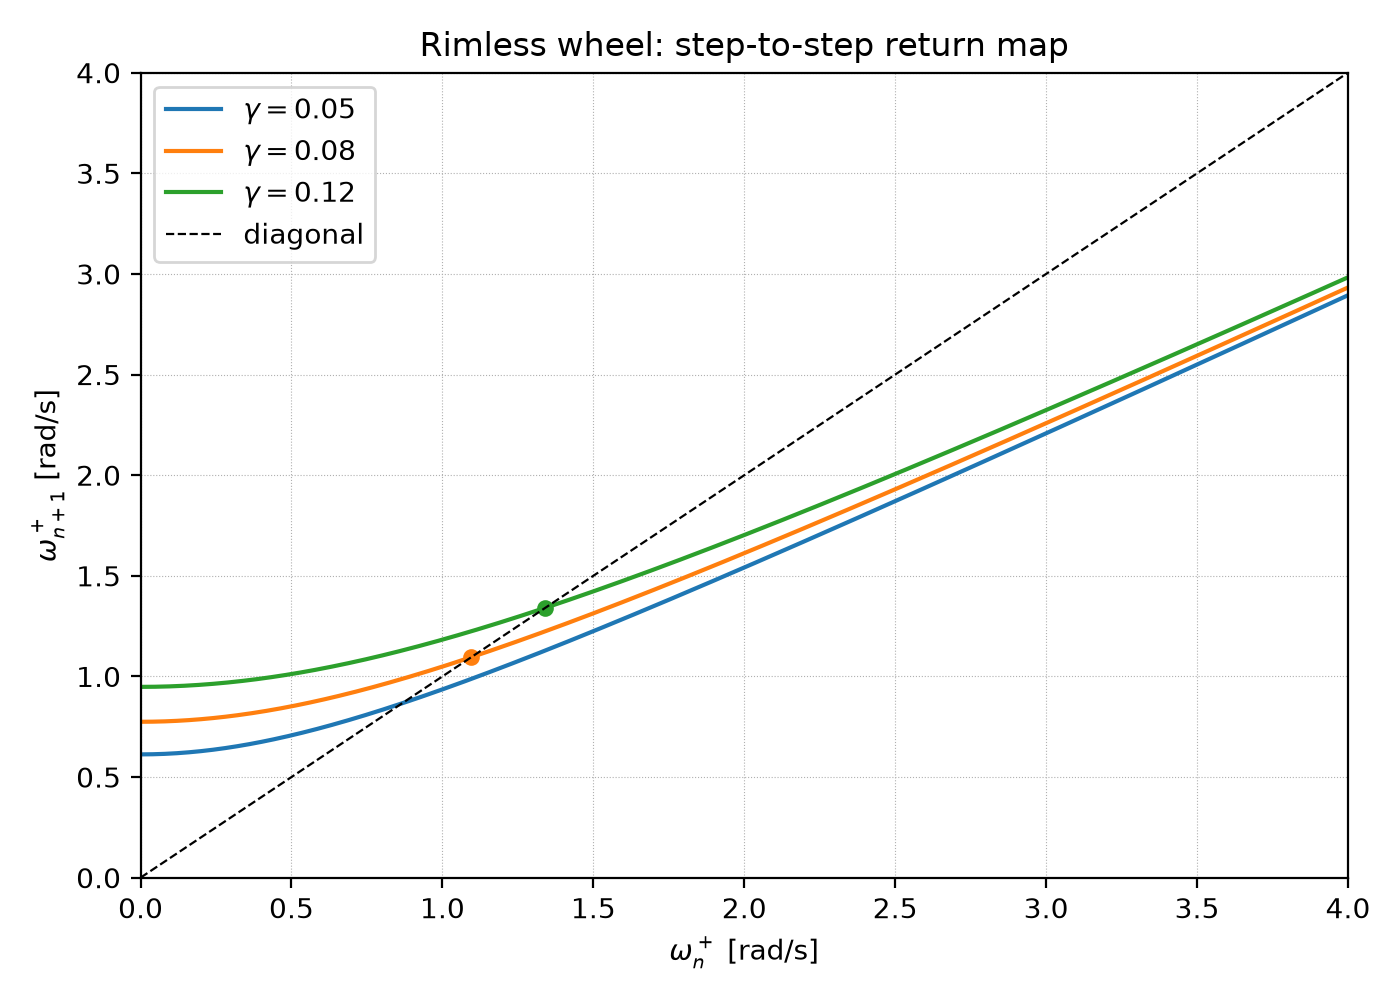
\includegraphics[width=0.72\textwidth]{fig_rw_return_map.png}
  \caption{Rimless wheel return map for three slopes.  Intersections with the
  diagonal are fixed points; only fixed points above the step threshold
  $\omega_1$ correspond to a sustained rolling gait.}
\end{figure}

\begin{figure}[htbp]
  \centering
  \begin{subfigure}{0.48\textwidth}
    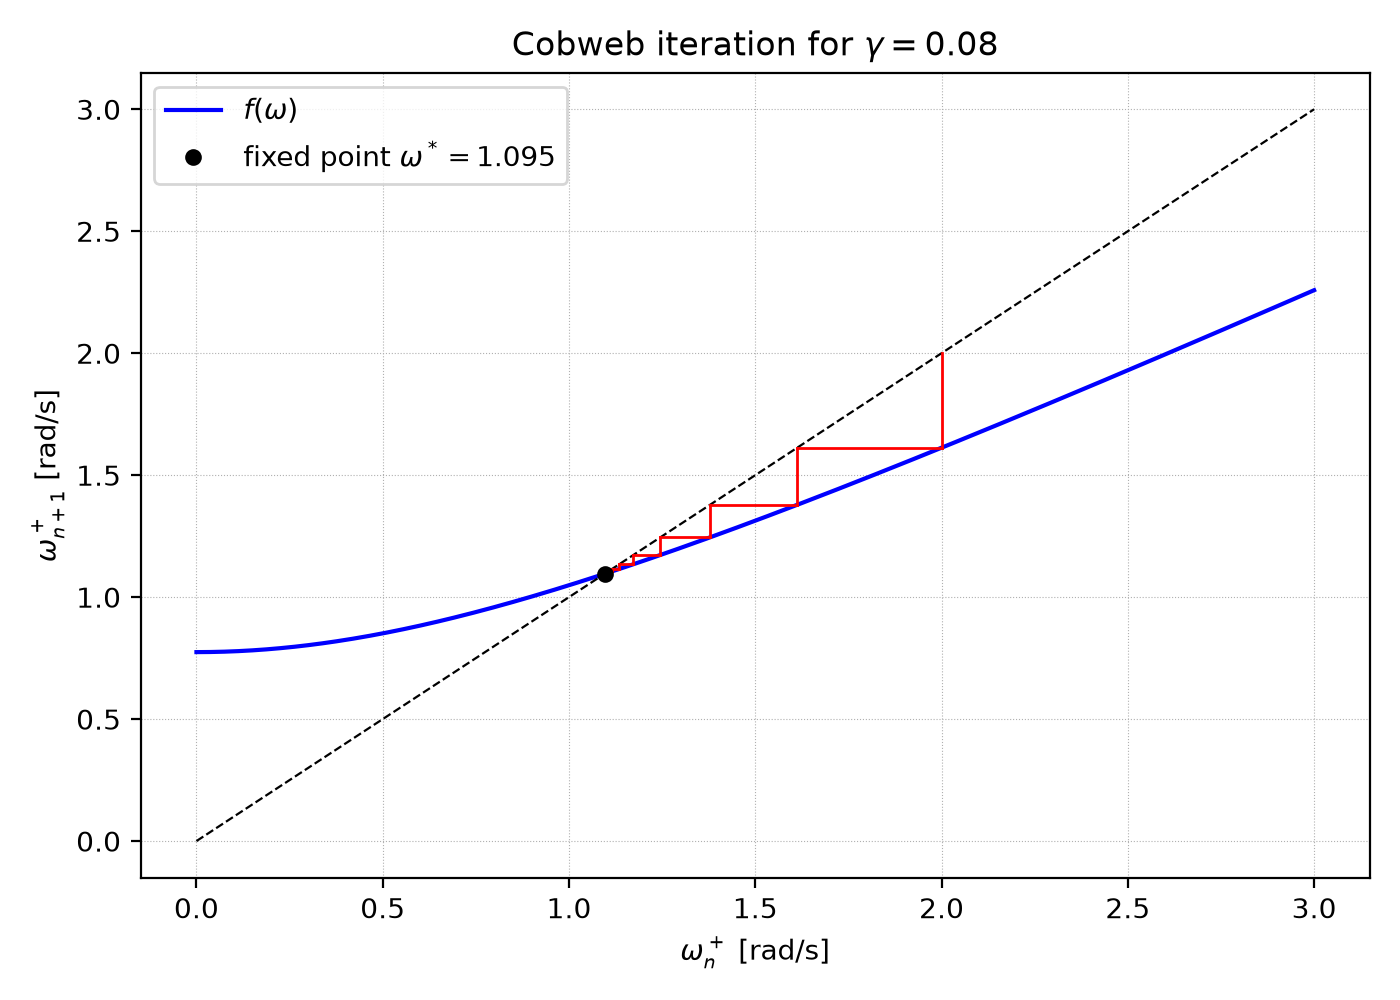
\includegraphics[width=\textwidth]{fig_rw_cobweb.png}
    \caption{Cobweb iteration at $\gamma=0.08$.}
  \end{subfigure}\hfill
  \begin{subfigure}{0.48\textwidth}
    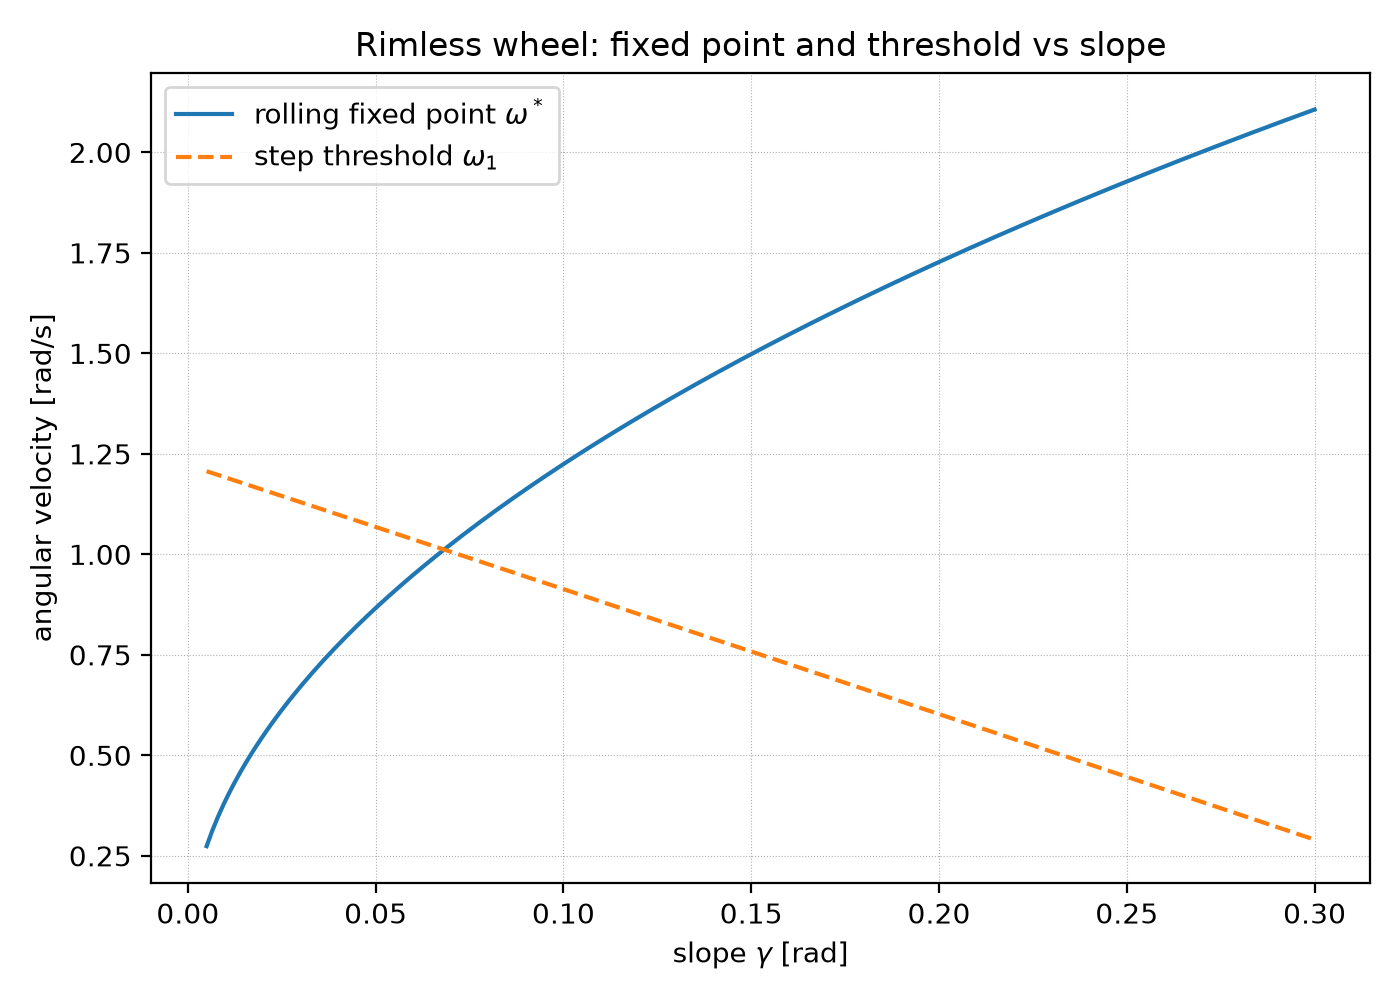
\includegraphics[width=\textwidth]{fig_rw_fixed_point.png}
    \caption{Fixed point and threshold vs.\ slope.}
  \end{subfigure}
  \caption{Rimless wheel: convergence to the stable fixed point and the
  existence condition $\omega^*>\omega_1$.}
\end{figure}

\subsection{What was run and sensitivity study}

The supplied notebook was run for initial angular velocities
$5,10,0.95,-5,-4.8$ rad/s.  Large positive velocities produce a rapid forward
rolling gait; a small positive velocity stops before passing the upright
position and swings back; negative velocities produce backward or oscillatory
motion.  This is exactly the three-branch structure of the return map in the
lecture notes.

\begin{table}[H]
\centering
\caption{Rimless wheel: threshold, fixed point and existence condition.}
\begin{tabular}{ccccc}
\toprule
$\gamma$ [rad] & $\omega_1$ [rad/s] & $\omega^*$ [rad/s] &
$\omega^*>\omega_1$? & $f'(\omega^*)$ \\
\midrule
0.02 & 1.1606 & 0.5480 & No & 0.5 \\
0.05 & 1.0681 & 0.8663 & No & 0.5 \\
0.08 & 0.9754 & 1.0955 & Yes & 0.5 \\
0.12 & 0.8515 & 1.3408 & Yes & 0.5 \\
0.20 & 0.6026 & 1.7272 & Yes & 0.5 \\
\bottomrule
\end{tabular}
\end{table}

\textbf{Comments.}  The wheel is a passive-dynamic walker: there is no
actuation.  Gravity supplies energy during each stance phase, and the
inelastic collision removes energy at each step.  A stable periodic gait exists
when these two effects balance, i.e.\ when the rolling fixed point lies above
the step threshold.  On very shallow slopes ($\gamma\lesssim0.067$ rad in our
parameters) the fixed point is below $\omega_1$; the wheel cannot complete a
step and eventually settles into the standing/oscillating branch.  The
stability multiplier is always $1/2$, independent of slope: the stronger
dissipation at larger slopes is exactly compensated by the larger gravity
input, so the linearised step-to-step dynamics remain equally stable.  This is
a clean example of a limit cycle generated by a hybrid system with impact
dissipation.

%=====================================================================
\section{Example 4.4: The Compass Gait}
%=====================================================================

\subsection{Model and hybrid dynamics}

The compass gait consists of two point-mass legs of mass $m=5$ kg and length
$l=1$ m ($a=b=0.5$ m) connected at a hip of mass $m_h=10$ kg.  The minimal
state is
\begin{equation}
\bx=[\theta_{st},\theta_{sw},\dot\theta_{st},\dot\theta_{sw}]^\top .
\end{equation}
During stance the stance foot is pinned; during swing the swing leg moves
freely; at heel strike an inelastic collision occurs and the roles of the two
legs are swapped.  The textbook model walks downhill on a ramp of slope
$\gamma=0.0525$ rad.

\begin{figure}[htbp]
\centering
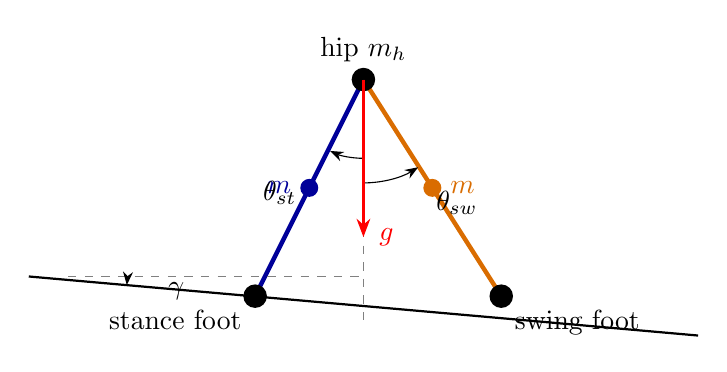
\begin{tikzpicture}[>=Stealth,scale=1.25]
  \draw[thick] (-3.4,0.3)--(3.4,-0.3);
  \coordinate (H) at (0,2.3);
  \coordinate (S) at (-1.1,0.1);
  \coordinate (W) at (1.4,0.1);
  \draw[ultra thick,blue!60!black] (H)--(S);
  \draw[ultra thick,orange!85!black] (H)--(W);
  \fill (H) circle (3.4pt) node[above=3pt] {hip $m_h$};
  \fill (S) circle (3.4pt) node[below left=2pt] {stance foot};
  \fill (W) circle (3.4pt) node[below right=2pt] {swing foot};
  \fill[blue!60!black] ($(H)!0.5!(S)$) circle (2.6pt) node[left=3pt] {$m$};
  \fill[orange!85!black] ($(H)!0.5!(W)$) circle (2.6pt) node[right=3pt] {$m$};
  \draw[dashed,gray] (H)--++(0,-2.5);
  \draw[->] (H)++(-90:0.80) arc[start angle=-90,end angle=-115,radius=0.80];
  \node at (-0.85,1.15) {$\theta_{st}$};
  \draw[->] (H)++(-90:1.05) arc[start angle=-90,end angle=-58,radius=1.05];
  \node at (0.95,1.05) {$\theta_{sw}$};
  \draw[->,thick,red] (H)--++(0,-1.6) node[right=2pt] {$g$};
  \draw[dashed,gray] (-3.0,0.3)--(0,0.3);
  \draw[->] (-2.4,0.3) arc[start angle=0,end angle=-5,radius=1.0];
  \node at (-1.9,0.15) {$\gamma$};
\end{tikzpicture}
\caption{Compass-gait schematic.  The stance leg is pinned at the ground;
the swing leg moves forward and becomes the next stance leg at heel strike.
The hip is a passive hinge in the example (zero torque), and each leg carries
a point mass $m$ at its center.}
\label{fig:compass_gait}
\end{figure}

\begin{intuition}[breakable=false,title={Why passive walking is possible, and why it is fragile}]
The compass gait has no motor.  Gravity pulls the body down the slope during
stance; the heel strike dissipates energy.  A periodic gait exists when the
two effects balance, just as for the rimless wheel.  The difference is that
the compass gait has only two legs and a free-swinging swing leg: the landing
geometry must match the previous step almost exactly.  This is why the basin
of attraction is a narrow band and why the same initial condition that works
on one slope can fail on another.  The step-to-step map is again the right
tool: a periodic gait is a fixed point, and its Floquet multipliers decide
whether a small perturbation decays.
\end{intuition}

\subsection{Results of the supplied notebook}

The notebook starts from $[0,0,0.4,-2.0]^\top$ with zero hip torque and runs
for 8 s.  The phase portrait (left leg angle vs.\ angular velocity) approaches
a closed orbit: the passive compass gait reaches a stable limit cycle.  The
impact at heel strike produces a visible jump in the velocity, while the
downhill slope replenishes the lost energy during the stance phase.

\begin{figure}[htbp]
  \centering
  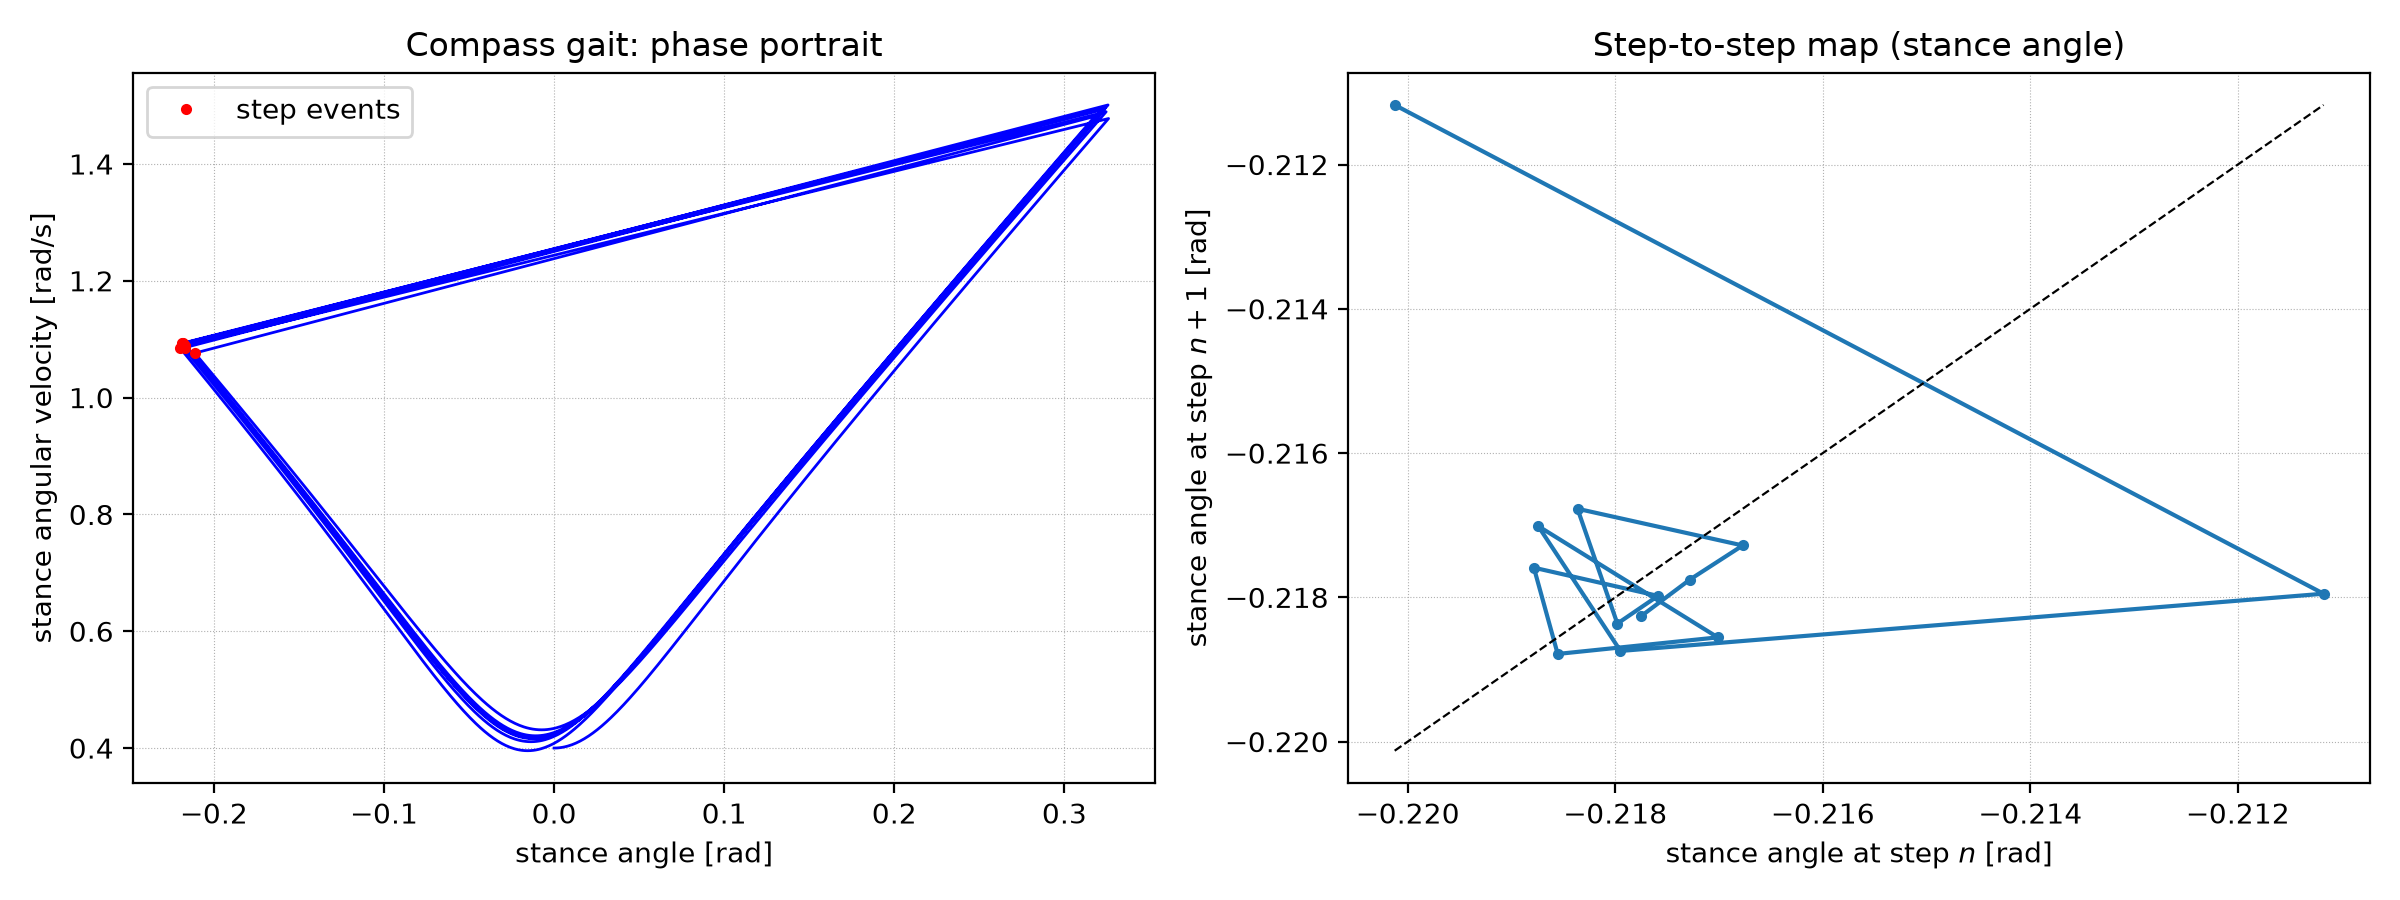
\includegraphics[width=0.9\textwidth]{fig_cg_phase.png}
  \caption{Compass gait: phase portrait (left) and step-to-step map of the
  stance angle (right).  Red dots mark the detected heel strikes; the points
  converge to a fixed point of the step map.}
\end{figure}

\subsection{Step detection and sensitivity}

We detect a step by a change of the plant's abstract ``left support'' state.
For the nominal initial condition the gait takes 14 steps in 10 s, with a mean
step period of 0.735 s.  The post-impact states converge rapidly to a
neighbourhood of the limit cycle.

\begin{figure}[htbp]
  \centering
  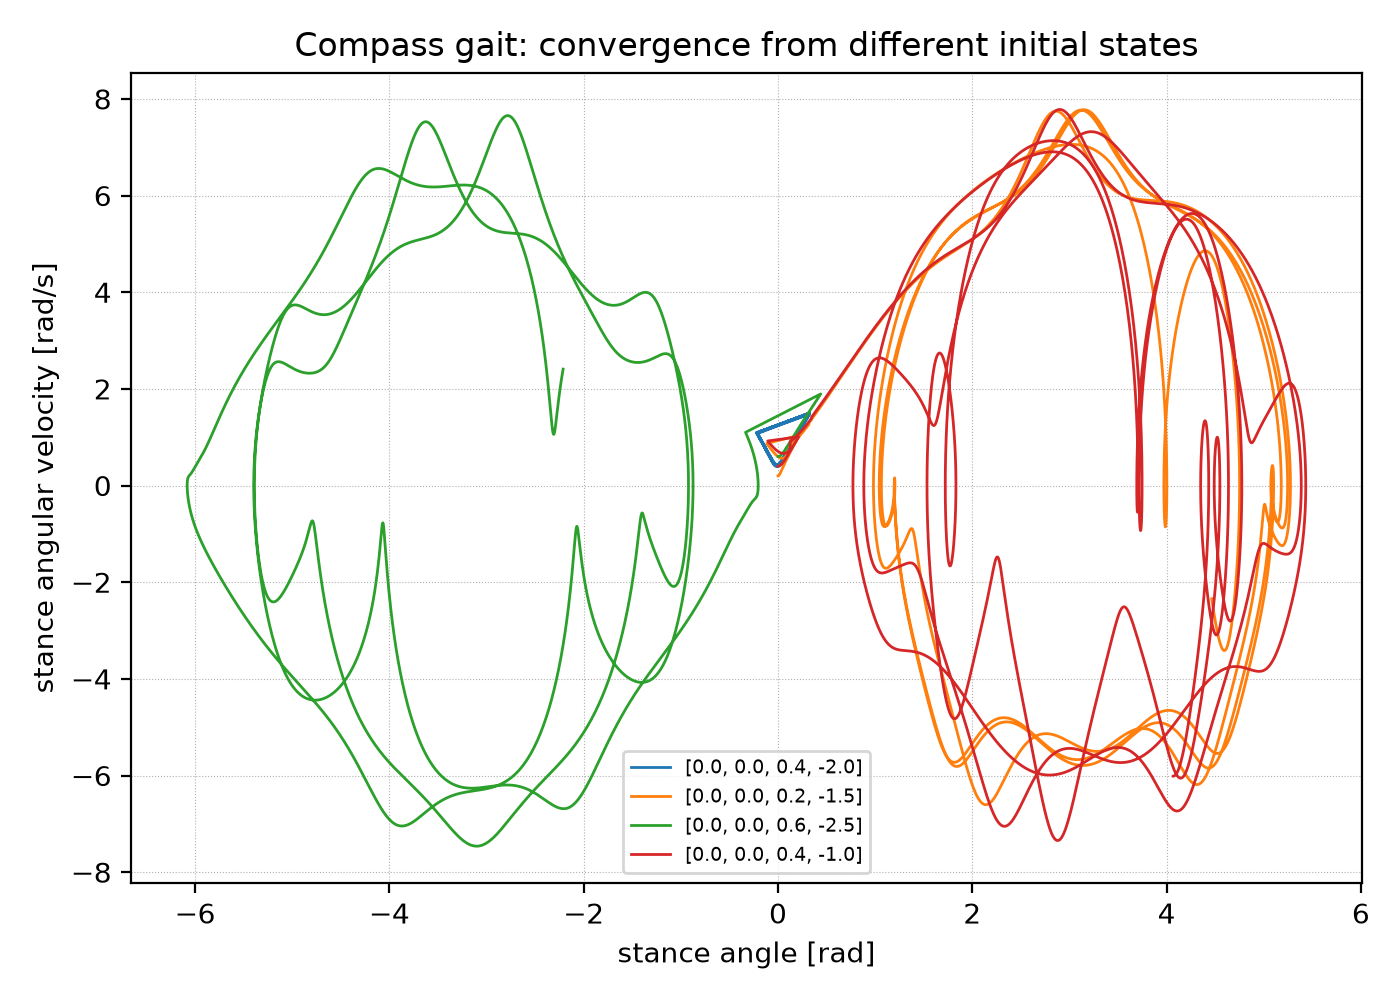
\includegraphics[width=0.72\textwidth]{fig_cg_initial.png}
  \caption{Compass gait from different initial states.  Only a limited set of
  initial conditions reaches the limit cycle; others leave the narrow basin
  and fall.}
\end{figure}

\begin{table}[H]
\centering
\caption{Compass gait: initial-condition sensitivity (10 s horizon).}
\begin{tabular}{ccc}
\toprule
Initial state & Steps & Bounded/sustained? \\
\midrule
$[0,0,0.4,-2.0]$ & 14 & Yes \\
$[0,0,0.2,-1.5]$ & 7 & No \\
$[0,0,0.6,-2.5]$ & 1 & No \\
$[0,0,0.4,-1.0]$ & 10 & No \\
\bottomrule
\end{tabular}
\end{table}

For the slope sensitivity we used a $3\times3$ grid of initial states
$\dot\theta_{st}(0)\in\{0.2,0.4,0.6\}$,
$\dot\theta_{sw}(0)\in\{-2.5,-2.0,-1.5\}$ and ran 12 s for each slope.  A run
is classified as sustained when it has at least 10 steps, the last five step
periods are consistent, and the state remains bounded.

\begin{table}[H]
\centering
\caption{Compass gait: fraction of initial states leading to a sustained gait.}
\begin{tabular}{cccc}
\toprule
Slope $\gamma$ [rad] & Successes / trials & Fraction & Mean period [s] \\
\midrule
0.0200 & 3/9 & 0.33 & 0.705 \\
0.0350 & 3/9 & 0.33 & 0.715 \\
0.0525 & 3/9 & 0.33 & 0.730 \\
0.0800 & 0/9 & 0.00 & -- \\
0.1200 & 0/9 & 0.00 & -- \\
\bottomrule
\end{tabular}
\end{table}

\begin{figure}[htbp]
  \centering
  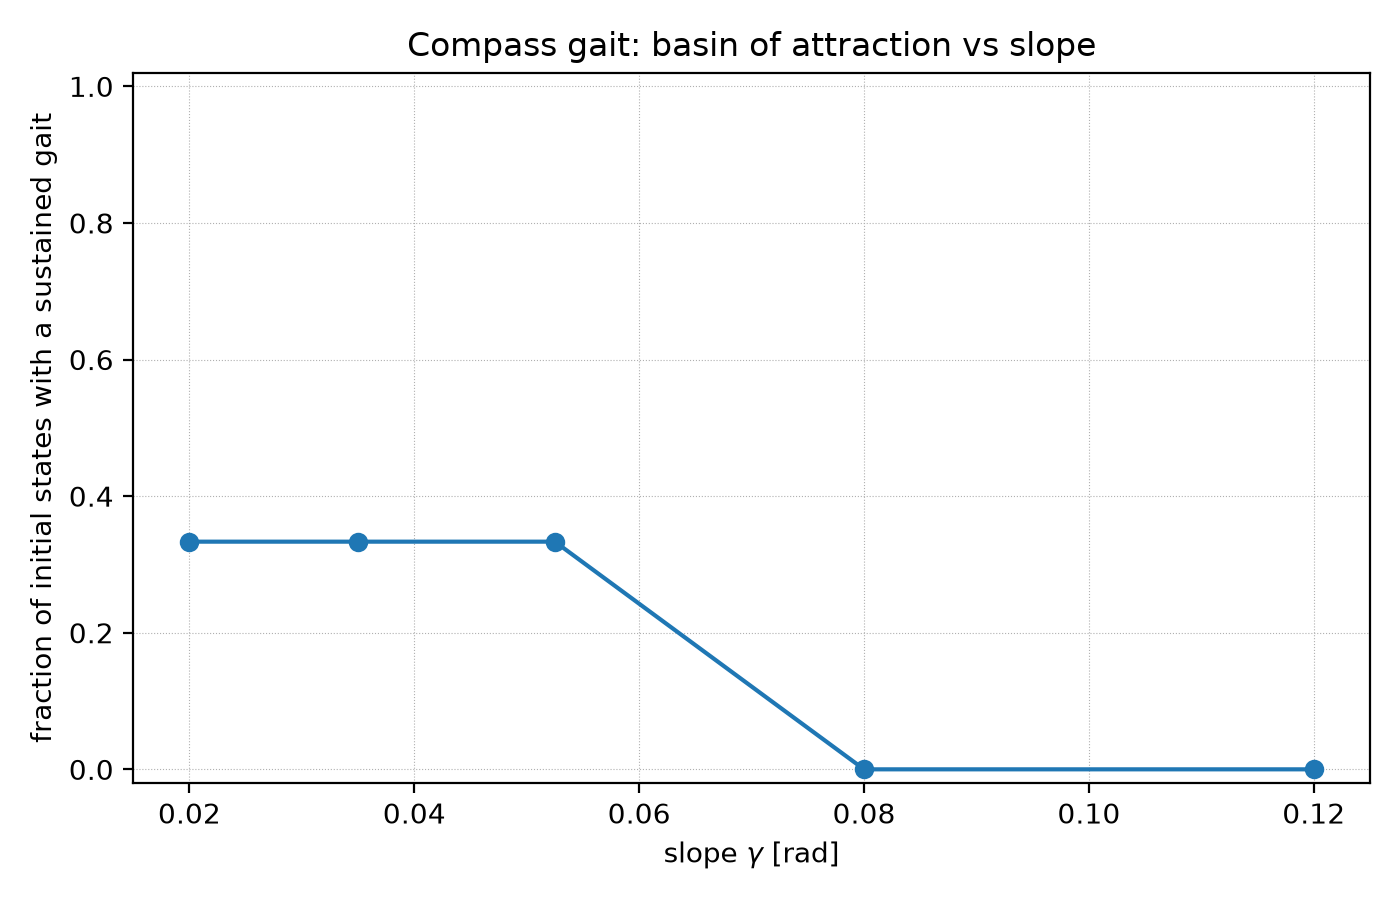
\includegraphics[width=0.65\textwidth]{fig_cg_slope.png}
  \caption{Compass gait: basin of attraction for the coarse initial-state grid
  as a function of slope.}
\end{figure}

\textbf{Comments.}  The compass gait is also passive: no hip torque is used.
Its limit cycle is an example of a stable periodic orbit of a hybrid system;
the step-to-step map plays the role of the Poincar\'e map and its linearised
eigenvalues (Floquet multipliers) determine orbital stability.  In contrast to
the rimless wheel, the basin of attraction is much narrower: only a small set
of initial conditions, and a limited range of slopes, leads to sustained
walking.  This is consistent with the lecture notes: with only two legs there
is no ``extra spoke'' to catch the body, so the swing-leg landing must be
timed precisely.  Real robots therefore need feedback (energy injection, foot
placement, posture control) to enlarge the basin.

%=====================================================================
\section{Example 4.5: The SLIP Model}
%=====================================================================

\subsection{Model}

The spring-loaded inverted pendulum (SLIP) models running with a point mass
$m=80$ kg, a massless spring leg of rest length $r_0=1$ m and stiffness
$k=10.7\,m g/r_0$, and a touchdown angle that can be reset during flight.
During flight the dynamics are ballistic:
\begin{equation}
\ddot x=0,\qquad
\ddot z=-g .
\end{equation}
During stance, with $r$ the leg length and $\theta$ the leg angle,
\begin{align}
m\ddot r-mr\dot\theta^2+mg\cos\theta-k(r_0-r)&=0,\\
mr^2\ddot\theta+2mr\dot r\dot\theta-mgr\sin\theta&=0 .
\end{align}
The total energy
\begin{equation}
E=\frac12m\left(\dot r^2+r^2\dot\theta^2\right)
+mgr\cos\theta+\frac12k(r_0-r)^2
\end{equation}
is conserved: there is no impact loss because the leg and foot are massless.
This is the key difference from the rimless wheel and compass gait.

\begin{figure}[htbp]
\centering
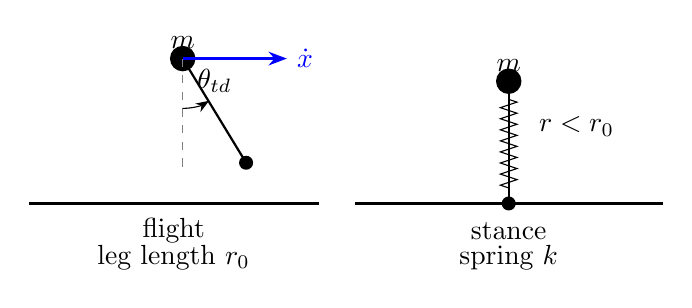
\begin{tikzpicture}[>=Stealth,scale=1.15]
  % flight
  \draw[thick] (-3.2,0)--(0,0);
  \coordinate (M) at (-1.5,1.6);
  \coordinate (F) at (-0.8,0.45);
  \draw[thick] (M)--(F);
  \fill (M) circle (4pt) node[above] {$m$};
  \fill (F) circle (2.2pt);
  \draw[dashed,gray] (M)--++(0,-1.2);
  \draw[->] (M)++(-90:0.55) arc[start angle=-90,end angle=-58,radius=0.55];
  \node at ($(M)+(0.35,-0.25)$) {$\theta_{td}$};
  \draw[->,blue,thick] (M)--++(1.15,0) node[right] {$\dot x$};
  \node at (-1.6,-0.30) {flight};
  \node at (-1.6,-0.60) {leg length $r_0$};
  % stance
  \draw[thick] (0.4,0)--(3.8,0);
  \coordinate (M2) at (2.1,1.35);
  \coordinate (F2) at (2.1,0);
  \draw[thick] (M2)--(F2);
  \draw[decoration={zigzag,segment length=4pt,amplitude=3pt},decorate]
       (2.1,1.15)--(2.1,0.15);
  \fill (M2) circle (4pt) node[above] {$m$};
  \fill (F2) circle (2.2pt);
  \node at (2.85,0.85) {$r<r_0$};
  \node at (2.1,-0.30) {stance};
  \node at (2.1,-0.60) {spring $k$};
\end{tikzpicture}
\caption{SLIP schematic.  In flight the leg is reset to the touchdown angle
$\theta_{td}$; in stance the spring compresses ($r<r_0$), stores energy and
extends again.  The leg and foot are massless, so there is no impulsive
energy loss at touchdown.}
\label{fig:slip}
\end{figure}

\begin{intuition}[breakable=false,title={Why SLIP is a ``conservative'' runner}]
The leg and foot are massless, so the ground contact does not produce an
impulse and the mechanical energy is conserved.  That is the main difference
from the rimless wheel and the compass gait, which lose energy at every
impact.  Running is therefore a segmented Hamiltonian motion: ballistic
flight, then a spring-mass stance, then flight again.  The touchdown angle
decides how much horizontal velocity is converted into compression.  Because
the energy is constant, the apex-to-apex map can be reduced to one dimension
on an energy slice, but that also limits what the map can prove.
\end{intuition}

\subsection{Results of the supplied notebook}

The notebook starts from a flight state with touchdown angle
$\theta_{td}=30^\circ$, dimensionless energy $\tilde E=1.61$ and apex height
$z=0.9$ m, and simulates 2 s.  The leg compresses during stance, stores elastic
energy, and extends again; the body follows a running-like trajectory with a
flight phase between stance phases.  The notebook also builds the
apex-to-apex map, which is analysed in the next section.

\textbf{Comments.}  SLIP is a segmented Hamiltonian system.  Unlike the
walking models, it has no dissipative impact, so the energy is constant to
integration accuracy.  The stance phase is a spring-mass oscillator with
centrifugal and gravity terms; the touchdown angle selects how much of the
horizontal velocity is converted into compression.  The model captures the
essential running mechanism (compression and restitution) while remaining low
dimensional.

%=====================================================================
\section{Example 4.6: The SLIP Apex-to-Apex Map}
%=====================================================================

\subsection{Poincar\'e section and one-dimensional map}

At the apex the vertical velocity is zero and the horizontal position is
irrelevant because of translation symmetry.  Energy conservation makes the
horizontal velocity a function of the apex height,
\begin{equation}
\dot x=\sqrt{\frac{2}{m}\left(E-mgz\right)},
\end{equation}
so the return map on the constant-energy slice is one-dimensional:
\begin{equation}
z[n+1]=P(z[n]).
\end{equation}
A fixed point $z^*=P(z^*)$ corresponds to a periodic running gait; its
stability is determined by $P'(z^*)$ (stable if $|P'|<1$).

\begin{figure}[htbp]
  \centering
  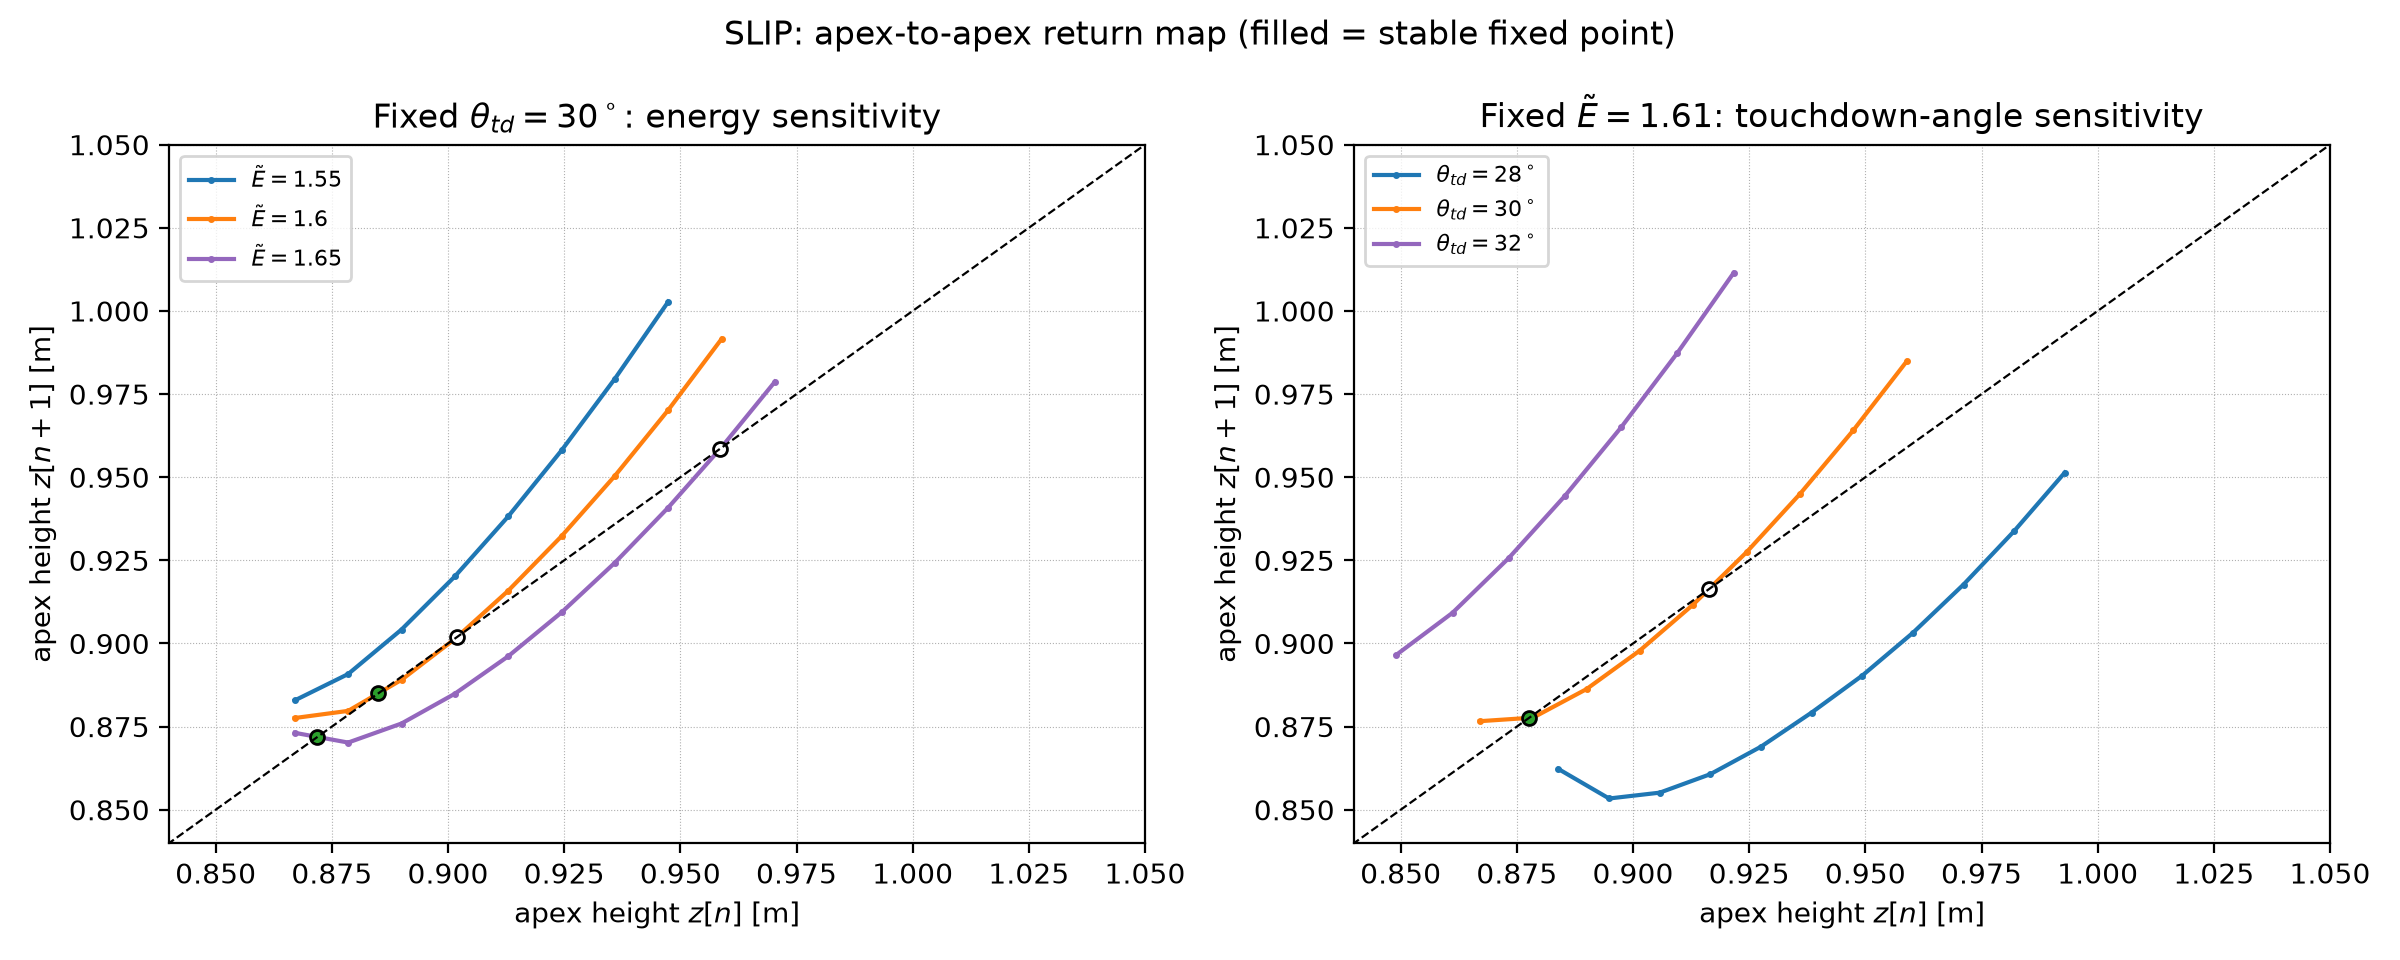
\includegraphics[width=0.95\textwidth]{fig_slip_map.png}
  \caption{SLIP apex-to-apex map.  Left: fixed touchdown angle
  $\theta_{td}=30^\circ$, varying energy.  Right: fixed energy
  $\tilde E=1.61$, varying touchdown angle.  Filled circles are stable fixed
  points, open circles are unstable ones.}
\end{figure}

\begin{figure}[htbp]
\centering
\begin{tikzpicture}[>=Stealth,scale=1.05]
  \draw[->] (0,0)--(6.4,0) node[right] {$z[n]$};
  \draw[->] (0,0)--(0,6.0) node[above] {$z[n+1]$};
  \draw[dashed,gray] (0,0)--(5.8,5.8);
  \draw[thick,blue] plot[domain=0.5:5.4,samples=100]
       (\x,{0.20*(\x-2.2)*(\x-3.8)+\x});
  \fill (2.2,2.2) circle (3.4pt)
       node[below right=2pt] {stable $z^\star$};
  \fill[white,draw=black] (3.8,3.8) circle (3.4pt)
       node[above left=2pt] {unstable $z_u$};
  \draw[->,red] (1.1,1.1)--(1.55,1.55);
  \draw[->,red] (2.9,2.9)--(2.45,2.45);
  \draw[->,red] (4.4,4.4)--(4.8,4.8);
\end{tikzpicture}
\caption{Schematic of a one-dimensional apex map.  Intersections of the blue
curve with the diagonal are periodic gaits.  A stable fixed point has
$|P'(z^\star)|<1$ (nearby iterates move toward it); an unstable one has
$|P'(z_u)|>1$.  The red arrows show the direction of the iteration.}
\label{fig:apex_map}
\end{figure}

\begin{recipe}[breakable=false,title={How to build and read a Poincar\'e map}]
\begin{enumerate}[leftmargin=1.4em,itemsep=2pt]
  \item Choose a section that the periodic orbit crosses once per cycle
        (e.g.\ the apex for SLIP, or the heel strike for walking).
  \item Simulate from many initial conditions on the section and record the
        next crossing.  This defines the map $z[n+1]=P(z[n])$.
  \item Find fixed points by solving $P(z)=z$; the slope $P'(z)$ at the fixed
        point decides stability ($|P'|<1$).
  \item Remember what the map projects away.  If it was obtained by using a
        conserved quantity, as in SLIP, the stability is only partial.
\end{enumerate}
\end{recipe}

\begin{pitfall}[breakable=false,title={A stable apex map is not full stability}]
For SLIP the map is computed on a constant-energy slice: the horizontal
velocity at the apex is reconstructed from $z$ and the total energy.  A
perturbation that changes the energy, such as a step in the terrain or a push,
is not represented by the one-dimensional map.  Thus $|P'|<1$ proves
stability only within that slice.  This is why the notes call it
\emph{partial} stability, and why a real robot still needs energy regulation.
\end{pitfall}

\subsection{Fixed points and sensitivity}

For the nominal condition $\theta_{td}=30^\circ$, $\tilde E=1.61$ we find
\begin{equation}
z^*_{\rm stable}=0.8776,\quad P'(z^*)=0.420,
\qquad
z^*_{\rm unstable}=0.9163,\quad P'(z^*)=1.288 .
\end{equation}
These agree with the textbook values ($0.8768$ and $0.9168$, with derivatives
$0.488$ and $1.346$); the small differences come from the finite grid and
linear interpolation.

\begin{table}[H]
\centering
\caption{SLIP: fixed points for the tested parameter neighbourhood.}
\begin{tabular}{cccc}
\toprule
$\theta_{td}$ [deg] & $\tilde E$ & $z^*$ [m] & $P'(z^*)$ \\
\midrule
30 & 1.60 & 0.8850 & 0.500 (stable) \\
30 & 1.60 & 0.9019 & 1.167 (unstable) \\
30 & 1.61 & 0.8776 & 0.420 (stable) \\
30 & 1.61 & 0.9163 & 1.288 (unstable) \\
30 & 1.65 & 0.8719 & 0.122 (stable) \\
30 & 1.65 & 0.9586 & 1.513 (unstable) \\
\bottomrule
\end{tabular}
\end{table}

\textbf{Comments.}  The apex map has a stable and an unstable fixed point for
the nominal parameters; initial heights between them converge to the lower
(stable) gait, while heights above the unstable point leave the map's domain
or fail.  Changing the energy by $\pm0.05$ moves the fixed points but leaves a
stable gait; changing the touchdown angle to $28^\circ$ or $32^\circ$ removes
the fixed point in our scan.  The stable fixed point at the nominal condition
is therefore a narrow operating point, consistent with the map's limited
domain.

\textbf{Partial stability.}  The one-dimensional map is obtained by projecting
the two-dimensional apex state $(z,\dot x)$ onto $z$ using energy
conservation.  Consequently, $|P'|<1$ only proves stability with respect to
perturbations that preserve the total energy.  It does not prove stability to
terrain changes, pushes or other disturbances that change the energy.  Since
SLIP is conservative, this is a \emph{partial} stability result, not asymptotic
stability of the full running motion.  This distinction is important for
control design: the apex map is useful for one-step-ahead controllers, but a
real robot needs additional energy regulation.

%=====================================================================
\section{Section 4.6: The One-Dimensional Hopper}
%=====================================================================

\subsection{Model and hopping cycle}

The hopper has a body of mass $m_b$ and a leg of mass $m_l$ connected by an
elastic prismatic joint of stiffness $k$.  With $z_b$ the body height and
$l=z_l-z_b$ the leg compression, the state is
$[z_b,l,\dot z_b,\dot l]^\top$.  The spring force is $-k(l+\delta)$, where
$\delta\ge0$ is the preload control.

The cycle has four phases: flight, touchdown (inelastic impact of the leg), the
stance phase (leg on the ground, body moving down and up), and lift-off
(inelastic impact between body and leg).  The controller changes $\delta$ only
twice per cycle:
\begin{itemize}[leftmargin=1.4em]
  \item at the bottom $t_{bt}$: set $\delta(t_{bt}^+)=\bar\delta$;
  \item at the apex $t_{ap}$: reset $\delta(t_{ap}^+)=0$.
\end{itemize}

\begin{figure}[htbp]
\centering
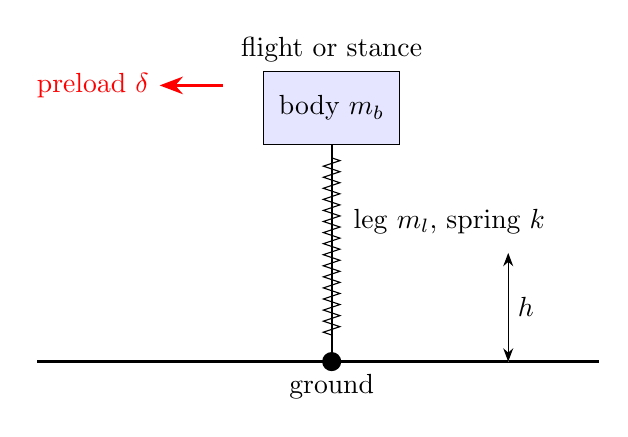
\begin{tikzpicture}[>=Stealth,scale=1.15]
  \draw[thick] (-1.0,0)--(5.2,0);
  \draw[fill=blue!10,draw=black] (1.5,2.4) rectangle (3.0,3.2);
  \node at (2.25,2.8) {body $m_b$};
  \coordinate (B) at (2.25,2.4);
  \coordinate (F) at (2.25,0.0);
  \draw[thick] (B)--(F);
  \draw[decoration={zigzag,segment length=4pt,amplitude=3pt},decorate]
       (2.25,2.25)--(2.25,0.25);
  \fill (F) circle (3pt);
  \node at (3.55,1.55) {leg $m_l$, spring $k$};
  \node at (2.25,-0.28) {ground};
  \draw[dashed,gray] (4.2,0)--(4.2,1.2);
  \draw[<->] (4.2,0)--(4.2,1.2) node[midway,right] {$h$};
  \draw[->,very thick,red] (1.05,3.05)--(0.35,3.05)
       node[left] {preload $\delta$};
  \node at (2.25,3.45) {flight or stance};
\end{tikzpicture}
\caption{One-dimensional hopper schematic.  The body and leg are connected
by a spring; $\delta\ge0$ is the preload.  The controller changes $\delta$
only at the bottom (apply $\bar\delta$) and at the apex (reset to zero).}
\label{fig:hopper}
\end{figure}

\begin{intuition}[breakable=false,title={The controller in one sentence}]
The collisions at touchdown and lift-off remove energy.  At the bottom of the
stance phase we compress the spring by a preload $\bar\delta$; this injects
exactly enough energy so that the next apex reaches the desired height $h$.
At the apex we reset the preload to zero.  The whole controller is therefore
a scalar energy calculation, updated twice per hop, not a trajectory tracker.
\end{intuition}

\subsection{Energy derivation of the preload}

The mechanical energy is
\begin{equation}
E=\frac12m_b\dot z_b^2+\frac12m_l(\dot z_b+\dot l)^2
+m_bg z_b+m_lg(z_b+l)+\frac12k(l+\delta)^2 .
\end{equation}
Before the preload is applied at the bottom, $l=-z_b$ and $\dot z_b=0$:
\begin{equation}
E(t_{bt}^-)=m_bg z_b+\frac12k z_b^2 .
\end{equation}
After applying $\bar\delta$,
\begin{equation}
E(t_{bt}^+)=m_bg z_b+\frac12k(\bar\delta-z_b)^2 .
\end{equation}
At lift-off, the body is at the hard stop and the leg is on the ground.  Water
energy conservation from bottom to lift-off gives the body kinetic energy
before impact:
\begin{equation}
\frac12m_b\dot z_b^2(t_{lo}^-)
=m_bg z_b+\frac12k z_b^2-k\bar\delta z_b .
\end{equation}
Momentum conservation for the inelastic lift-off impact gives
\begin{equation}
E(t_{lo}^+)=\frac{m_b}{m_b+m_l}
\left[m_bg z_b+\frac12k z_b^2-k\bar\delta z_b\right]
+\frac12k\bar\delta^2 .
\end{equation}
At the apex both body and leg are at rest at height $h$:
\begin{equation}
E(t_{ap}^-)=(m_b+m_l)gh+\frac12k\bar\delta^2 .
\end{equation}
Since energy is conserved during flight, $E(t_{lo}^+)=E(t_{ap}^-)$, which
gives the linear equation for $\bar\delta$:
\begin{equation}
\boxed{
\bar\delta=\frac12z_b+\frac{m_bg}{k}
-\frac{(m_b+m_l)^2}{k m_b z_b}gh .
}
\end{equation}
If this value is negative, the system already has too much energy; the
controller then uses $\bar\delta=0$ and lets the impacts remove energy.

\subsection{Implementation}

\begin{lstlisting}[language=Python,caption={Mechanical energy of the hopper.}]
def mechanical_energy(state, delta):
    k, mb, ml, g = get_hopper_parameters()
    zb, l, zb_dot, l_dot = state
    zl_dot = zb_dot + l_dot
    E = (0.5 * mb * zb_dot**2 + 0.5 * ml * zl_dot**2
         + mb * g * zb + ml * g * (zb + l)
         + 0.5 * k * (l + delta)**2)
    return np.asarray(E)
\end{lstlisting}

\begin{lstlisting}[language=Python,caption={Preload controller.}]
class PreloadController(LeafSystem):
    def __init__(self, h):
        LeafSystem.__init__(self)
        self.DeclareVectorInputPort("state", 4)
        self.DeclareVectorOutputPort("delta", 1, self.DoCalcVectorOutput)
        self.h = h
        self.hopper_parameters = get_hopper_parameters()
        self.last_delta = 0.0
        self.last_state = np.full(4, np.nan)

    def is_bottom_or_apex(self, state):
        if np.any(np.isnan(self.last_state)):
            return None
        zb, l, zb_dot, l_dot = state
        last_zb_dot = self.last_state[2]
        if last_zb_dot <= 0.0 and zb_dot > 0.0:
            return "bottom" if zb < 0.0 else "apex"
        if last_zb_dot >= 0.0 and zb_dot < 0.0:
            return "apex" if zb > 0.0 else "bottom"
        return None

    def get_delta_bar(self, state):
        k, mb, ml, g = self.hopper_parameters
        zb = state[0]
        return (0.5 * zb + mb * g / k
                - ((mb + ml) ** 2) * g * self.h / (k * mb * zb))

    def DoCalcVectorOutput(self, context, delta):
        state = self.get_input_port(0).Eval(context)
        event = self.is_bottom_or_apex(state)
        if event == "bottom":
            delta.SetFromVector([max(self.get_delta_bar(state), 0.0)])
        elif event == "apex":
            delta.SetFromVector([0.0])
        else:
            delta.SetFromVector([self.last_delta])
        self.last_delta = delta[0]
        self.last_state = np.array(state)
\end{lstlisting}

\subsection{Results and autograding}

The notebook was executed end-to-end.  The autograder reports
\begin{center}
\textbf{Total score is 13/13: mechanical energy 3/3, preload controller 10/10.}
\end{center}

\begin{figure}[H]
  \centering
  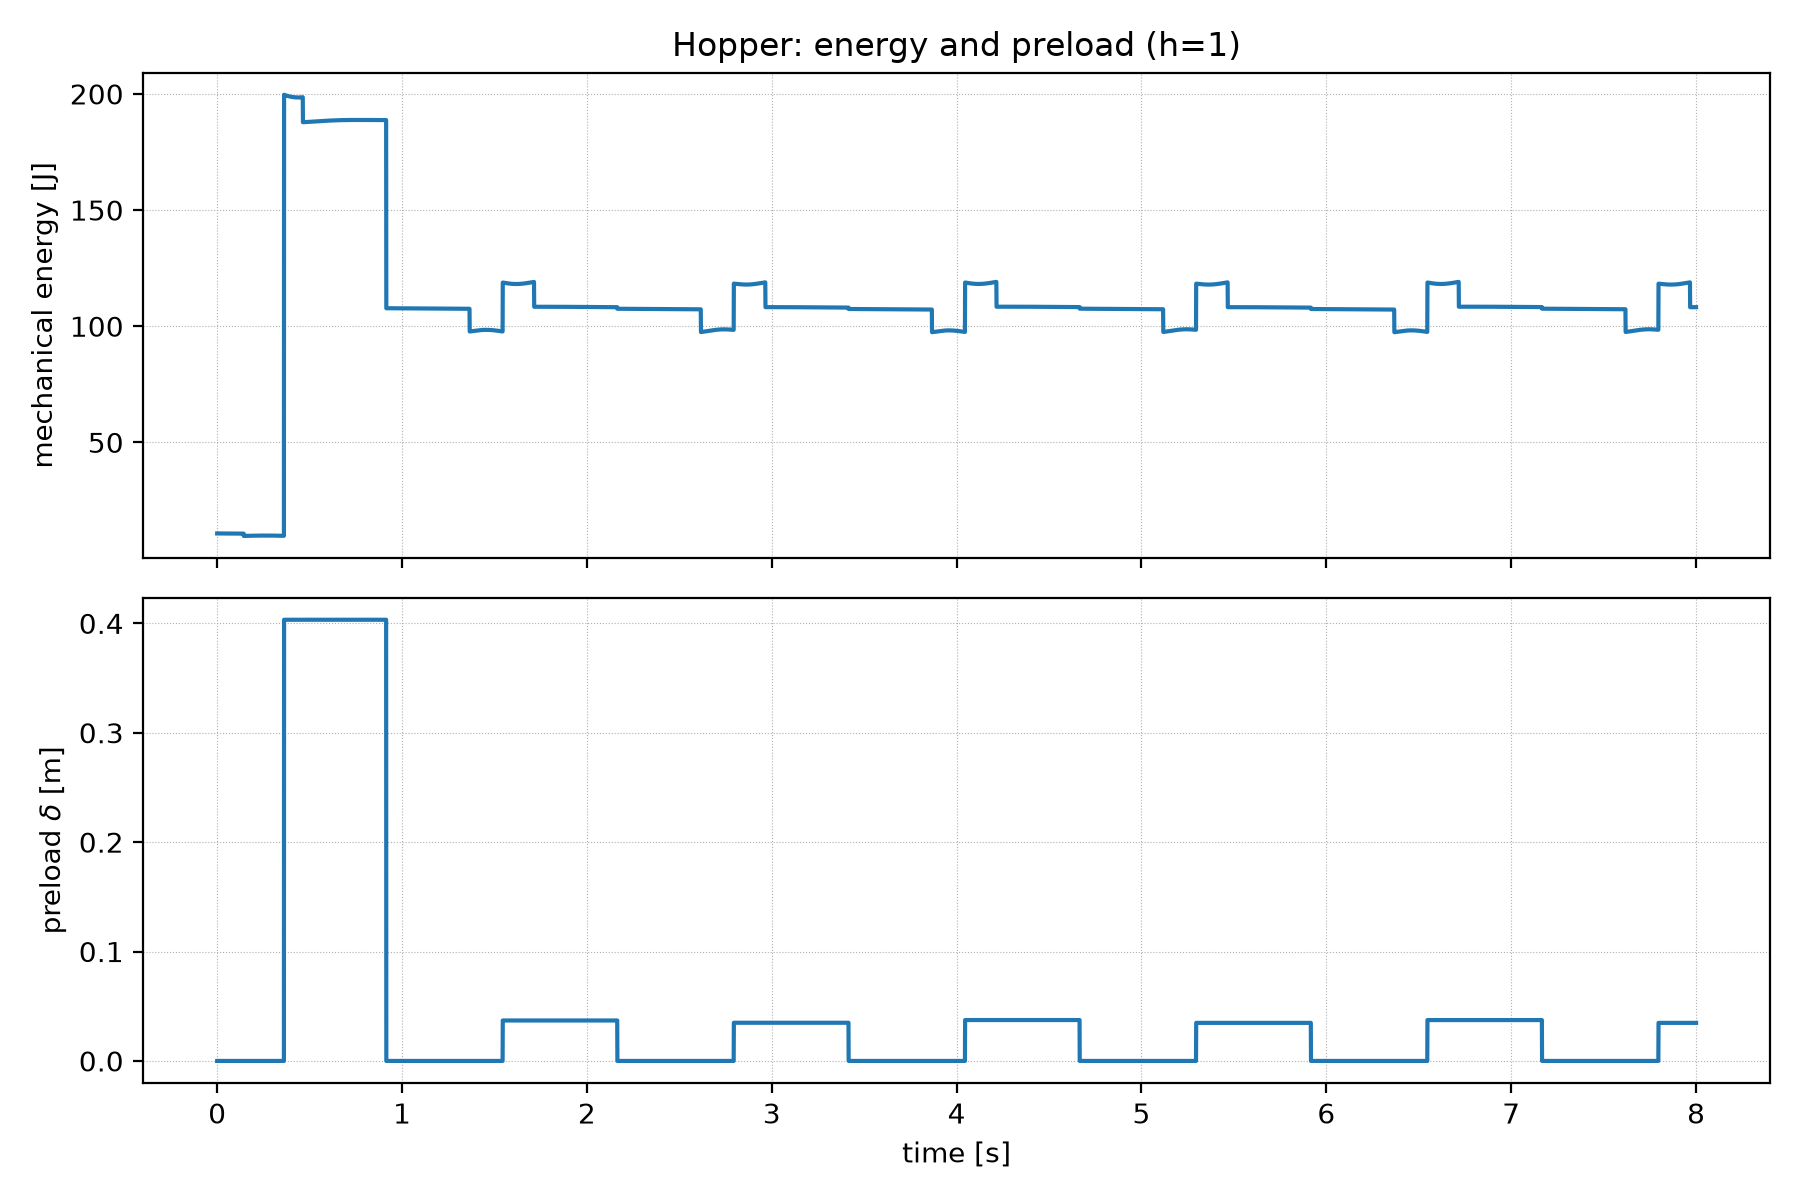
\includegraphics[width=0.9\textwidth]{fig_hopper_energy.png}
  \caption{Hopper energy and preload for $h=1$ m.  The preload is applied at
  the bottom and reset at the apex; the energy drops at the two impacts.}
\end{figure}

\begin{table}[H]
\centering
\caption{Hopper: target-height sensitivity (final 2 s of an 8 s run).}
\begin{tabular}{cccc}
\toprule
Target $h$ [m] & Max body height [m] & Error [m] & Max preload $\delta$ [m] \\
\midrule
0.50 & 0.4985 & $-0.0015$ & 0.024 \\
0.75 & 0.7477 & $-0.0023$ & 0.093 \\
1.00 & 0.9966 & $-0.0034$ & 0.163 \\
1.25 & 1.2444 & $-0.0056$ & 0.232 \\
1.50 & 1.4946 & $-0.0054$ & 0.302 \\
\bottomrule
\end{tabular}
\end{table}

\begin{table}[H]
\centering
\caption{Hopper: initial-height sensitivity for $h=1$ m.}
\begin{tabular}{cccc}
\toprule
Initial $z_b(0)$ [m] & Max height (last 2 s) [m] & Error [m] & Max preload [m] \\
\midrule
0.1 & 0.9966 & $-0.0034$ & 0.403 \\
0.3 & 0.9966 & $-0.0034$ & 0.247 \\
0.5 & 0.9966 & $-0.0034$ & 0.163 \\
0.8 & 0.9966 & $-0.0034$ & 0.078 \\
1.0 & 0.9966 & $-0.0034$ & 0.037 \\
\bottomrule
\end{tabular}
\end{table}

\begin{figure}[H]
  \centering
  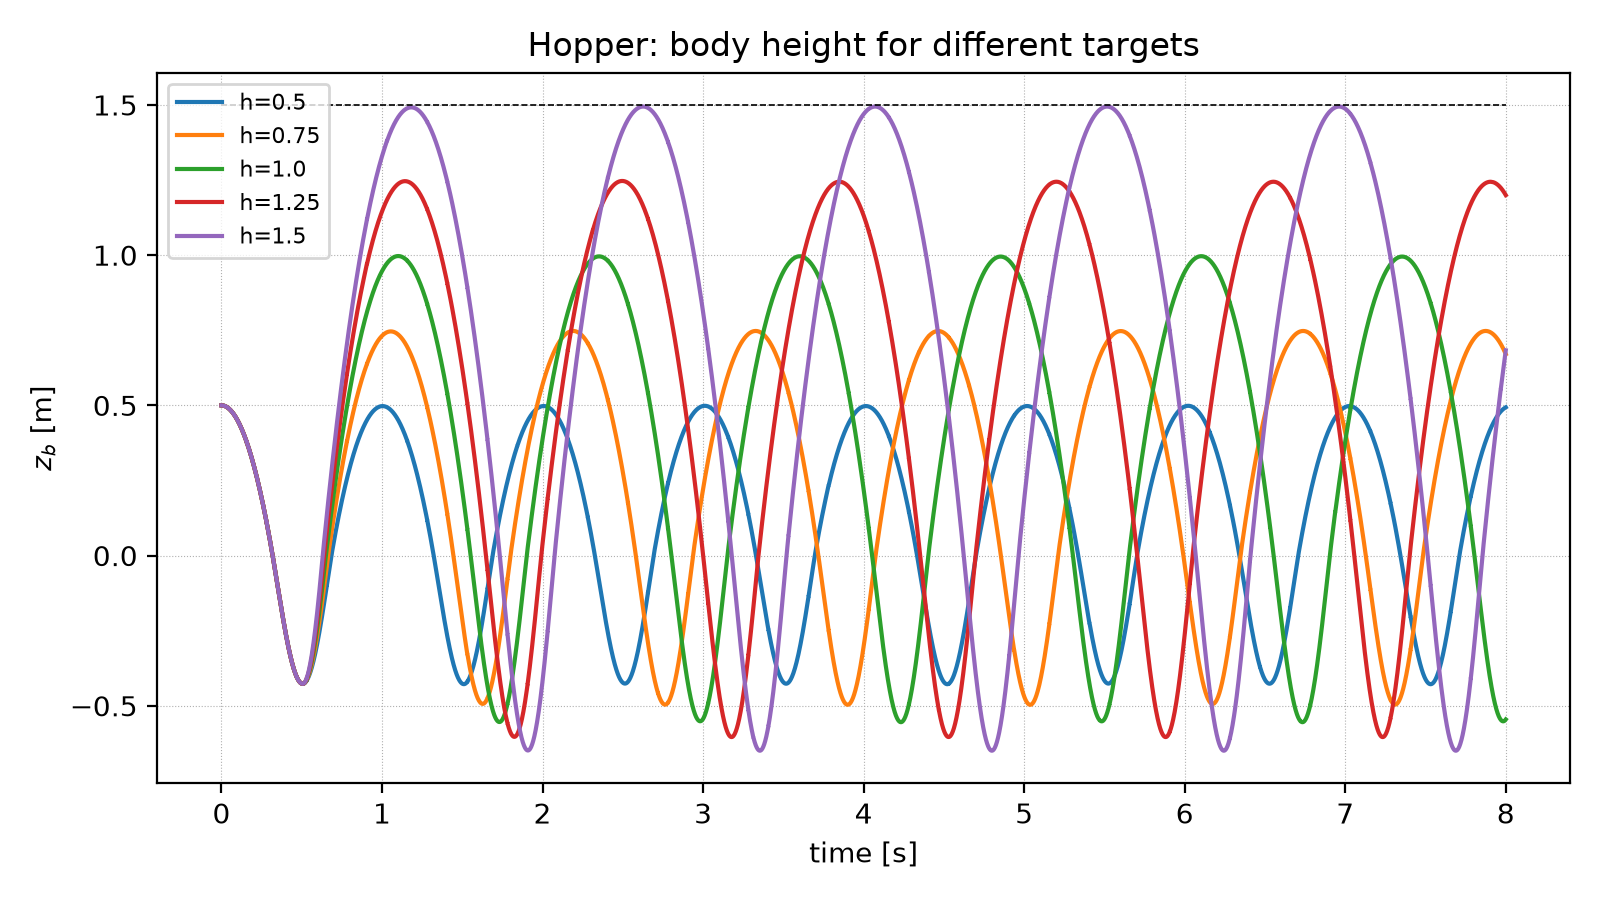
\includegraphics[width=0.9\textwidth]{fig_hopper_height.png}
  \caption{Hopper: body height for different target heights.  After a short
  transient all runs settle into a periodic hop at the requested height.}
\end{figure}

\begin{figure}[H]
  \centering
  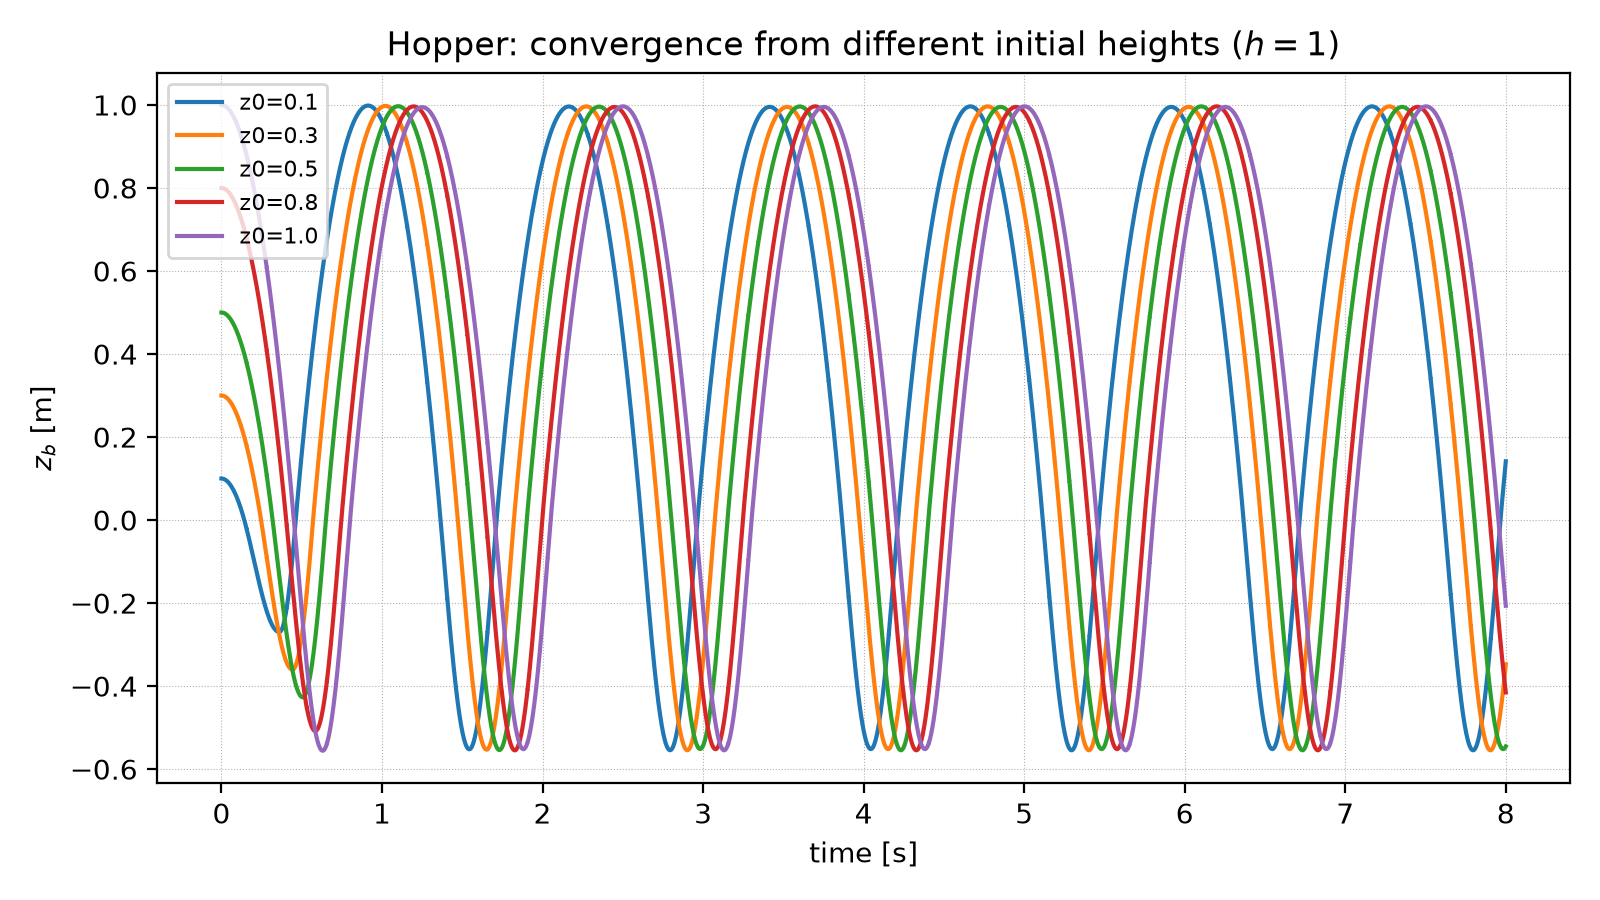
\includegraphics[width=0.9\textwidth]{fig_hopper_initial.png}
  \caption{Hopper: convergence from different initial body heights at
  $h=1$ m.  The energy controller rejects the initial-height error.}
\end{figure}

\textbf{Comments.}  The controller is an energy-based one-step controller: it
does not track a reference trajectory, but chooses the preload exactly so that
the next apex has the desired mechanical energy.  The target-height error is
below 6 mm for all tested heights, and the controller is insensitive to the
initial body height.  The maximum preload grows roughly linearly with the
target height: a higher hop needs more energy, and the spring stores it as
$\frac12k\bar\delta^2$.  The initial transient is larger when the hopper starts
low, because more energy must be injected at the first bottom; after that the
cycle is periodic.  This is a clean example of using a Poincar\'e/energy
argument to reduce a trajectory-tracking problem to a scalar control decision
once per hopping cycle.

%=====================================================================
\section{Conclusions}
%=====================================================================

\begin{enumerate}[leftmargin=1.4em]
  \item \textbf{Passive dynamic walking.}  The rimless wheel and the compass
  gait show that a stable periodic gait can arise without actuation: gravity
  supplies energy during stance and collisions remove it at foot strike.  The
  step-to-step return map is the natural tool; its fixed point is the gait and
  its slope/Floquet multipliers determine orbital stability.
  \item \textbf{Rimless wheel.}  The return map is one-dimensional and the
  fixed point is stable with multiplier $\cos^2(2\alpha)=1/2$.  The main
  sensitivity is the slope: below a critical slope the fixed point lies below
  the step threshold and no rolling gait exists.
  \item \textbf{Compass gait.}  The limit cycle is much more delicate: only a
  narrow set of initial conditions and slopes leads to sustained walking.  The
  coarse sensitivity grid confirms the small basin of attraction; feedback is
  needed for robustness.
  \item \textbf{SLIP.}  The model is conservative and captures running as a
  sequence of flight and spring stance phases.  The apex map has a stable and
  an unstable fixed point for the nominal parameters, but the one-dimensional
  stability is only partial because it relies on energy conservation.  The
  touchdown angle and energy strongly affect whether a fixed point exists.
  \item \textbf{Hopper.}  The energy analysis gives a closed-form preload
  $\bar\delta(z_b,h)$; the controller applies it at the bottom and resets at
  the apex.  The autograder passes 13/13, the hopping height error is below
  6 mm, and the controller is robust to the initial body height.
\end{enumerate}

%=====================================================================
\section{Code and Reproduction}\label{sec:repro}
%=====================================================================

The complete code is in the repository.  Main entry points:
\begin{center}
\small
\begin{tabular}{ll}
\toprule
Topic & Script / notebook \\
\midrule
Example 4.3 & \texttt{Exp4'3-rimless-wheel.ipynb}, \texttt{rimless\_wheel\_analysis.py} \\
Example 4.4 & \texttt{Exp4'4-compass-gait.ipynb}, \texttt{compass\_gait\_analysis.py} \\
Examples 4.5/4.6 & \texttt{Exp4'5-6-slip.ipynb}, \texttt{slip\_analysis.py} \\
Section 4.6 & \texttt{Exp4'6-one\_d\_hopper.ipynb}, \texttt{one\_d\_hopper\_analysis.py} \\
\bottomrule
\end{tabular}
\end{center}

Commands (from \texttt{Ch-4/exp4\_analysis}):
\begin{lstlisting}[language=bash]
/Users/leo/venvs/drake/bin/python rimless_wheel_analysis.py
/Users/leo/venvs/drake/bin/python compass_gait_analysis.py
/Users/leo/venvs/drake/bin/python slip_analysis.py
/Users/leo/venvs/drake/bin/python one_d_hopper_analysis.py
\end{lstlisting}

Headless notebook execution:
\begin{lstlisting}[language=bash]
COLAB_TESTING=1 /Users/leo/venvs/drake/bin/jupyter nbconvert \
  --to notebook --execute --inplace --ExecutePreprocessor.timeout=300 \
  "Exp4'6-one_d_hopper.ipynb"
\end{lstlisting}

The report is compiled with
\begin{lstlisting}[language=bash]
pdflatex Ch4_Report.tex
pdflatex Ch4_Report.tex
\end{lstlisting}

\appendix
\section{Key Code Snippets}

\subsection{Rimless wheel return map}

\begin{lstlisting}[language=Python]
def f_map(omega, gamma):
    return np.cos(2 * ALPHA) * np.sqrt(
        np.maximum(omega**2 + D(gamma), 0.0))

def fixed_point(gamma):
    return (1.0 / np.tan(2 * ALPHA)) * np.sqrt(D(gamma))
\end{lstlisting}

\subsection{SLIP apex map}

\begin{lstlisting}[language=Python]
def apex_map(touchdown_angle, Etilde, n=30, zmax=1.2):
    plant = SpringLoadedInvertedPendulum()
    s = SLIPState(np.zeros(8))
    s.theta = touchdown_angle
    s.r = 1.0
    simulator = Simulator(plant)
    context = simulator.get_mutable_context()
    plant.get_input_port(0).FixValue(context, [touchdown_angle])
    context.SetAccuracy(1e-5)
    zs = np.linspace(np.cos(touchdown_angle) + 0.001, zmax, n)
    zns = np.full(n, np.nan)
    for i, z in enumerate(zs):
        s.z = z
        s.xdot = plant.apex_velocity_from_dimensionless_system_energy(Etilde, z)
        context.SetTime(0.0)
        context.get_mutable_continuous_state_vector().SetFromVector(s[:])
        simulator.Initialize()
        simulator.AdvanceTo(0.6)
        if plant.last_apex is not None:
            zns[i] = plant.last_apex
        plant.last_apex = None
    return zs, zns
\end{lstlisting}

\end{document}
